\documentclass{standalone}
\usepackage{tikz}
\usetikzlibrary{patterns, positioning}


\begin{document}
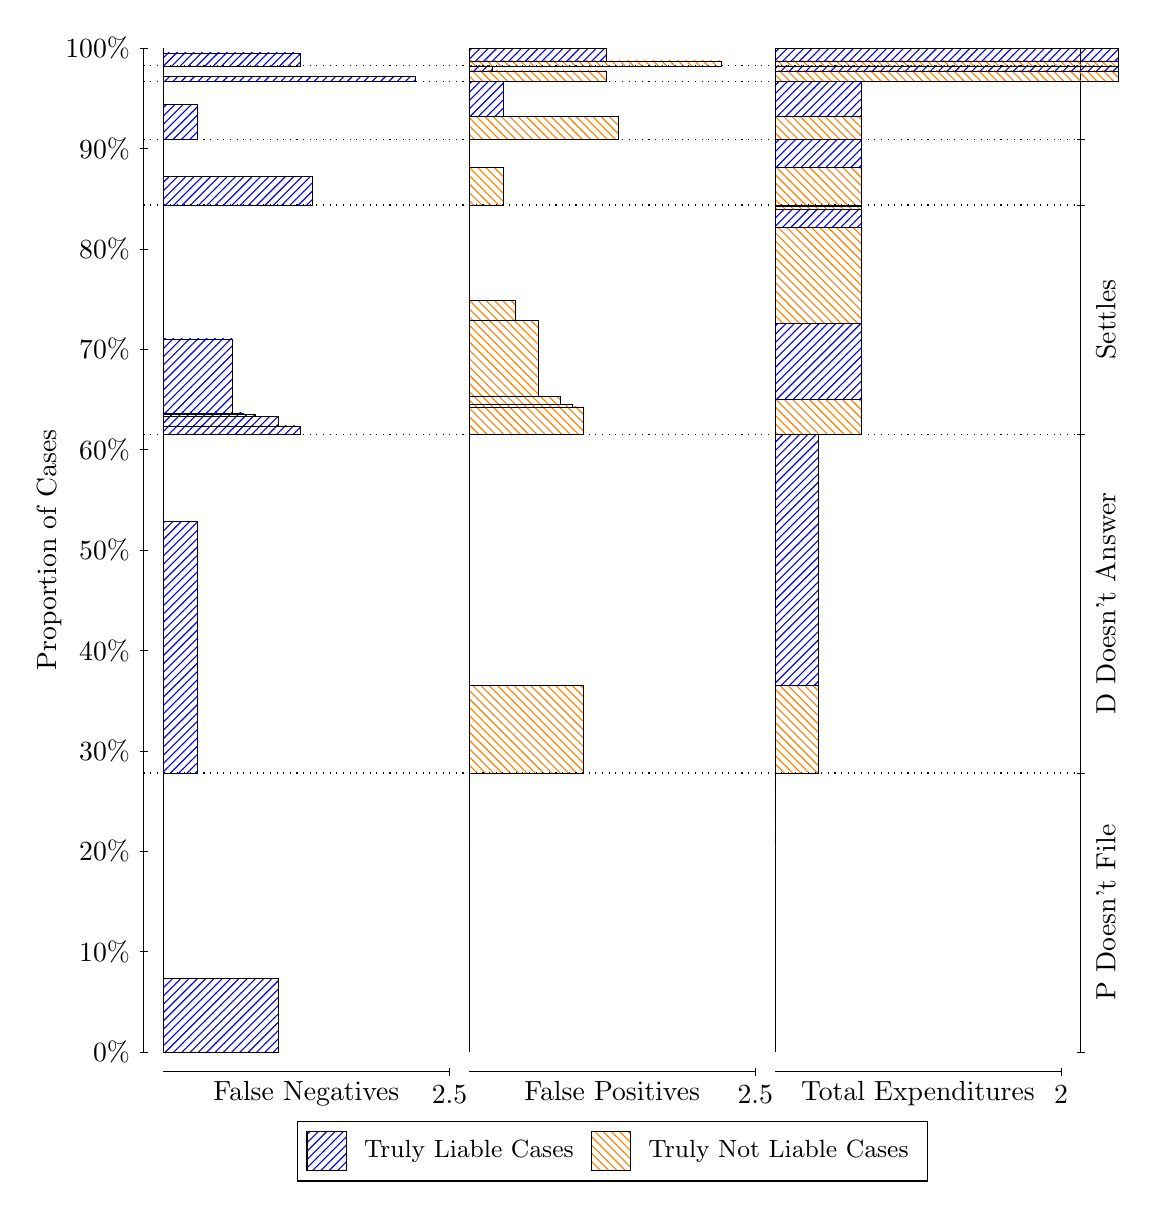
\begin{tikzpicture}
\draw[black, very thin] (1.5,1.75) -- (1.5,14.5);
\node[rotate=90, text=black, anchor=center] at (0.3, 8.125) {Proportion of Cases};
\draw[black, very thin] (1.45,1.75) -- (1.55,1.75);
\node[text=black, anchor=east] at (1.45, 1.75) {0\%};
\draw[black, very thin] (1.45,3.025) -- (1.55,3.025);
\node[text=black, anchor=east] at (1.45, 3.025) {10\%};
\draw[black, very thin] (1.45,4.3) -- (1.55,4.3);
\node[text=black, anchor=east] at (1.45, 4.3) {20\%};
\draw[black, very thin] (1.45,5.575) -- (1.55,5.575);
\node[text=black, anchor=east] at (1.45, 5.575) {30\%};
\draw[black, very thin] (1.45,6.85) -- (1.55,6.85);
\node[text=black, anchor=east] at (1.45, 6.85) {40\%};
\draw[black, very thin] (1.45,8.125) -- (1.55,8.125);
\node[text=black, anchor=east] at (1.45, 8.125) {50\%};
\draw[black, very thin] (1.45,9.4) -- (1.55,9.4);
\node[text=black, anchor=east] at (1.45, 9.4) {60\%};
\draw[black, very thin] (1.45,10.675) -- (1.55,10.675);
\node[text=black, anchor=east] at (1.45, 10.675) {70\%};
\draw[black, very thin] (1.45,11.95) -- (1.55,11.95);
\node[text=black, anchor=east] at (1.45, 11.95) {80\%};
\draw[black, very thin] (1.45,13.225) -- (1.55,13.225);
\node[text=black, anchor=east] at (1.45, 13.225) {90\%};
\draw[black, very thin] (1.45,14.5) -- (1.55,14.5);
\node[text=black, anchor=east] at (1.45, 14.5) {100\%};

\draw[black, very thin] (13.4,1.75) -- (13.4,14.5);
\draw[black, very thin] (13.35,1.75) -- (13.45,1.75);
\node[anchor=west] at (13.35, 1.75) {};
\draw[black, very thin] (13.35,5.2934) -- (13.45,5.2934);
\node[anchor=west] at (13.35, 5.2934) {};
\draw[black, very thin] (13.35,9.5969) -- (13.45,9.5969);
\node[anchor=west] at (13.35, 9.5969) {};
\draw[black, very thin] (13.35,12.506) -- (13.45,12.506);
\node[anchor=west] at (13.35, 12.506) {};
\draw[black, very thin] (13.35,13.343) -- (13.45,13.343);
\node[anchor=west] at (13.35, 13.343) {};
\draw[black, very thin] (13.35,14.076) -- (13.45,14.076);
\node[anchor=west] at (13.35, 14.076) {};
\draw[black, very thin] (13.35,14.273) -- (13.45,14.273);
\node[anchor=west] at (13.35, 14.273) {};
\draw[black, very thin] (13.35,14.5) -- (13.45,14.5);
\node[anchor=west] at (13.35, 14.5) {};

\draw[black, very thin, pattern color=blue, pattern=north east lines] (1.75,1.75) rectangle (3.2033,2.6864);
\draw[black, very thin, pattern color=orange, pattern=north west lines] (1.75,2.6864) rectangle (1.75,5.2934);
\draw[black, very thin, pattern color=blue, pattern=north east lines] (1.75,5.2934) rectangle (2.186,8.4893);
\draw[black, very thin, pattern color=orange, pattern=north west lines] (1.75,8.4893) rectangle (1.75,9.5969);
\draw[black, very thin, pattern color=blue, pattern=north east lines] (1.75,9.5969) rectangle (3.494,9.7002);
\draw[black, very thin, pattern color=blue, pattern=north east lines] (1.75,9.7002) rectangle (3.2033,9.822);
\draw[black, very thin, pattern color=blue, pattern=north east lines] (1.75,9.822) rectangle (2.9127,9.8455);
\draw[black, very thin, pattern color=blue, pattern=north east lines] (1.75,9.8455) rectangle (2.7673,9.8652);
\draw[black, very thin, pattern color=blue, pattern=north east lines] (1.75,9.8652) rectangle (2.622,10.806);
\draw[black, very thin, pattern color=orange, pattern=north west lines] (1.75,10.806) rectangle (1.75,12.506);
\draw[black, very thin, pattern color=blue, pattern=north east lines] (1.75,12.506) rectangle (3.6393,12.868);
\draw[black, very thin, pattern color=orange, pattern=north west lines] (1.75,12.868) rectangle (1.75,13.343);
\draw[black, very thin, pattern color=blue, pattern=north east lines] (1.75,13.343) rectangle (2.186,13.787);
\draw[black, very thin, pattern color=orange, pattern=north west lines] (1.75,13.787) rectangle (1.75,14.076);
\draw[black, very thin, pattern color=blue, pattern=north east lines] (1.75,14.076) rectangle (4.9473,14.139);
\draw[black, very thin, pattern color=orange, pattern=north west lines] (1.75,14.139) rectangle (1.75,14.273);
\draw[black, very thin, pattern color=blue, pattern=north east lines] (1.75,14.273) rectangle (3.494,14.437);
\draw[black, very thin, pattern color=orange, pattern=north west lines] (1.75,14.437) rectangle (1.75,14.5);
\draw[black, very thin, pattern color=orange, pattern=north west lines] (5.6333,1.75) rectangle (5.6333,4.357);
\draw[black, very thin, pattern color=blue, pattern=north east lines] (5.6333,4.357) rectangle (5.6333,5.2934);
\draw[black, very thin, pattern color=orange, pattern=north west lines] (5.6333,5.2934) rectangle (7.0867,6.401);
\draw[black, very thin, pattern color=blue, pattern=north east lines] (5.6333,6.401) rectangle (5.6333,9.5969);
\draw[black, very thin, pattern color=orange, pattern=north west lines] (5.6333,9.5969) rectangle (7.0867,9.9418);
\draw[black, very thin, pattern color=orange, pattern=north west lines] (5.6333,9.9418) rectangle (6.9413,9.9773);
\draw[black, very thin, pattern color=orange, pattern=north west lines] (5.6333,9.9773) rectangle (6.796,10.075);
\draw[black, very thin, pattern color=orange, pattern=north west lines] (5.6333,10.075) rectangle (6.5053,11.039);
\draw[black, very thin, pattern color=orange, pattern=north west lines] (5.6333,11.039) rectangle (6.2147,11.297);
\draw[black, very thin, pattern color=blue, pattern=north east lines] (5.6333,11.297) rectangle (5.6333,12.506);
\draw[black, very thin, pattern color=orange, pattern=north west lines] (5.6333,12.506) rectangle (6.0693,12.981);
\draw[black, very thin, pattern color=blue, pattern=north east lines] (5.6333,12.981) rectangle (5.6333,13.343);
\draw[black, very thin, pattern color=orange, pattern=north west lines] (5.6333,13.343) rectangle (7.5227,13.632);
\draw[black, very thin, pattern color=blue, pattern=north east lines] (5.6333,13.632) rectangle (6.0693,14.076);
\draw[black, very thin, pattern color=orange, pattern=north west lines] (5.6333,14.076) rectangle (7.3773,14.21);
\draw[black, very thin, pattern color=blue, pattern=north east lines] (5.6333,14.21) rectangle (5.924,14.273);
\draw[black, very thin, pattern color=orange, pattern=north west lines] (5.6333,14.273) rectangle (8.8307,14.336);
\draw[black, very thin, pattern color=blue, pattern=north east lines] (5.6333,14.336) rectangle (7.3773,14.5);
\draw[black, very thin, pattern color=orange, pattern=north west lines] (9.5167,1.75) rectangle (9.5167,4.357);
\draw[black, very thin, pattern color=blue, pattern=north east lines] (9.5167,4.357) rectangle (9.5167,5.2934);
\draw[black, very thin, pattern color=orange, pattern=north west lines] (9.5167,5.2934) rectangle (10.062,6.401);
\draw[black, very thin, pattern color=blue, pattern=north east lines] (9.5167,6.401) rectangle (10.062,9.5969);
\draw[black, very thin, pattern color=orange, pattern=north west lines] (9.5167,9.5969) rectangle (10.607,10.04);
\draw[black, very thin, pattern color=blue, pattern=north east lines] (9.5167,10.04) rectangle (10.607,11.004);
\draw[black, very thin, pattern color=orange, pattern=north west lines] (9.5167,11.004) rectangle (10.607,12.226);
\draw[black, very thin, pattern color=blue, pattern=north east lines] (9.5167,12.226) rectangle (10.607,12.451);
\draw[black, very thin, pattern color=orange, pattern=north west lines] (9.5167,12.451) rectangle (10.607,12.486);
\draw[black, very thin, pattern color=blue, pattern=north east lines] (9.5167,12.486) rectangle (10.607,12.506);
\draw[black, very thin, pattern color=orange, pattern=north west lines] (9.5167,12.506) rectangle (10.607,12.981);
\draw[black, very thin, pattern color=blue, pattern=north east lines] (9.5167,12.981) rectangle (10.607,13.343);
\draw[black, very thin, pattern color=orange, pattern=north west lines] (9.5167,13.343) rectangle (10.607,13.632);
\draw[black, very thin, pattern color=blue, pattern=north east lines] (9.5167,13.632) rectangle (10.607,14.076);
\draw[black, very thin, pattern color=orange, pattern=north west lines] (9.5167,14.076) rectangle (13.877,14.21);
\draw[black, very thin, pattern color=blue, pattern=north east lines] (9.5167,14.21) rectangle (13.877,14.273);
\draw[black, very thin, pattern color=orange, pattern=north west lines] (9.5167,14.273) rectangle (13.877,14.336);
\draw[black, very thin, pattern color=blue, pattern=north east lines] (9.5167,14.336) rectangle (13.877,14.5);
\draw[black, dotted] (1.5,5.2934) -- (13.4,5.2934);
\draw[black, dotted] (1.5,9.5969) -- (13.4,9.5969);
\draw[black, dotted] (1.5,12.506) -- (13.4,12.506);
\draw[black, dotted] (1.5,13.343) -- (13.4,13.343);
\draw[black, dotted] (1.5,14.076) -- (13.4,14.076);
\draw[black, dotted] (1.5,14.273) -- (13.4,14.273);
\draw[black, very thin] (1.75,1.5) -- (5.3833,1.5);
\node[text=black, anchor=north] at (3.5667, 1.5) {False Negatives};
\draw[black, very thin] (5.3833,1.45) -- (5.3833,1.55);
\node[text=black, anchor=north] at (5.3833, 1.45) {2.5};

\draw[black, very thin] (5.6333,1.5) -- (9.2667,1.5);
\node[text=black, anchor=north] at (7.45, 1.5) {False Positives};
\draw[black, very thin] (9.2667,1.45) -- (9.2667,1.55);
\node[text=black, anchor=north] at (9.2667, 1.45) {2.5};

\draw[black, very thin] (9.5167,1.5) -- (13.15,1.5);
\node[text=black, anchor=north] at (11.333, 1.5) {Total Expenditures};
\draw[black, very thin] (13.15,1.45) -- (13.15,1.55);
\node[text=black, anchor=north] at (13.15, 1.45) {2};

\node[text=black, centered, rotate=90] at (13.72, 3.5217) {P Doesn't File};
\node[text=black, centered, rotate=90] at (13.72, 7.4452) {D Doesn't Answer};
\node[text=black, centered, rotate=90] at (13.72, 11.051) {Settles};





\draw (7.449999999999999,1.5) node[draw=none] (baseCoordinate) {};
\begin{scope}[align=center]
        \matrix[scale=0.5, draw=black, below=0.5cm of baseCoordinate, nodes={draw}, column sep=0.1cm]{
            \node[rectangle, draw, minimum width=0.5cm, minimum height=0.5cm, pattern color=blue, pattern=north east lines] {}; &
            \node[draw=none, font=\small, text=black] (B) {Truly Liable Cases}; &
            \node[rectangle, draw, minimum width=0.5cm, minimum height=0.5cm, pattern color=orange, pattern=north west lines] {}; &
            \node[draw=none, font=\small, text=black] (B) {Truly Not Liable Cases}; \\
            };
\end{scope}

\end{tikzpicture}
\end{document}